% Folie 1: Vom Wasserstoffatom zu Mehrelektronensystemen
\begin{frame}{Grundlagen atomarer Orbitale}
    \textbf{Wasserstoffatom (exakt lösbar):}
    \begin{itemize}
        \item Zeitunabhängige SG: $\left(-\frac{\hbar^2}{2\mu}\nabla^2 - \frac{e^2}{4\pi\epsilon_0 r}\right)\psi = E\psi$
        \item Lösung: $\psi_{nlm}(r,\theta,\phi) = R_{nl}(r)Y_l^m(\theta,\phi)$
        \item Quantenzahlen: $n,l,m$
    \end{itemize}

    \begin{columns}
        \column{0.5\textwidth}
        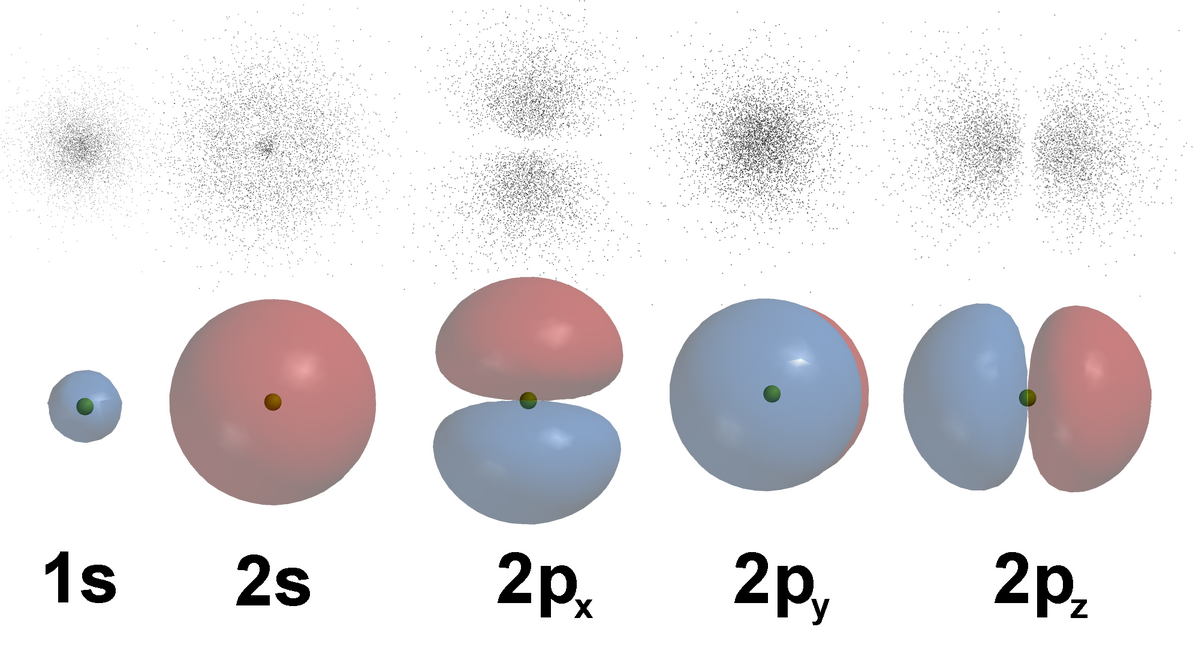
\includegraphics[width=\textwidth]{orbitals.png}

        \column{0.5\textwidth}
        \begin{itemize}
            \item Radialteil $R_{nl}(r)$
            \item Winkelteil $Y_l^m(\theta,\phi)$
        \end{itemize}
    \end{columns}
\end{frame}

% Folie 2: Das Mehrelektronenproblem
\begin{frame}{Die Herausforderung bei Mehrelektronenatomen}
    \textbf{Schrödinger-Gleichung:}
    \[
        \hat{H} = \sum_i \left(-\frac{\hbar^2}{2m}\nabla_i^2 - \frac{Ze^2}{4\pi\epsilon_0 r_i}\right) + \sum_{i<j} \frac{e^2}{4\pi\epsilon_0 r_{ij}}
    \]

    \begin{itemize}
        \item Elektron-Elektron-Wechselwirkung macht Gleichung unlösbar
        \item \alert{Approximationsmethoden} erforderlich:
        \begin{itemize}
            \item Hartree-Fock-Methode
            \item Dichtefunktionaltheorie (DFT)
        \end{itemize}
    \end{itemize}
\end{frame}

% Folie 3: Hartree-Fock-Methode
\begin{frame}{Hartree-Fock-Approximation}
    \textbf{Key Ideas:}
    \begin{itemize}
        \item Jedes Elektron bewegt sich im gemittelten Feld der anderen
        \item Slater-Determinante für Antisymmetrie
    \end{itemize}

    \textbf{Hartree-Fock-Gleichungen:}
    \[
        \hat{F}\phi_i(1) = \epsilon_i\phi_i(1)
    \]
    Fock-Operator:
    \[
        \hat{F} = \hat{h} + \sum_j (\hat{J}_j - \hat{K}_j)
    \]
    \begin{itemize}
        \item $\hat{J}_j$: Coulomb-Operator
        \item $\hat{K}_j$: Austauschoperator
    \end{itemize}
\end{frame}

% Folie 4: Dichtefunktionaltheorie
\begin{frame}{Dichtefunktionaltheorie (DFT)}
    \textbf{Hohenberg-Kohn-Theorem:}
    \begin{itemize}
        \item Grundzustandsenergie ist Funktional der Elektronendichte
        \item $E[n(\vec{r})] = T[n] + V_{ext}[n] + E_{ee}[n]$
    \end{itemize}

    \textbf{Kohn-Sham-Gleichungen:}
    \[
        \left(-\frac{\hbar^2}{2m}\nabla^2 + v_{eff}(\vec{r})\right)\psi_i = \epsilon_i\psi_i
    \]
    Effektives Potenzial:
    \[
        v_{eff} = v_{ext} + \int \frac{n(\vec{r}')}{|\vec{r}-\vec{r}'|}d\vec{r}' + v_{xc}[n]
    \]
\end{frame}

% Folie 5: Numerische Berechnung
\begin{frame}{Vom Konzept zur Berechnung}
    \textbf{Praktische Umsetzung:}
    \begin{itemize}
        \item Basis-Sätze (Gauß-Funktionen, planewaves)
        \item Selbstkonsistente Feld-Iteration
        \item Software-Pakete: Gaussian, VASP, Quantum ESPRESSO
    \end{itemize}

%    \begin{block}{Berechnungsschritte}
%        \begin{enumerate}
%            \item Start mit Trial-Dichte
%            \item Löse Kohn-Sham-Gleichungen
%            \item Aktualisiere Dichte
%            \item Wiederhole bis Konvergenz
%        \end{enumerate}
%    \end{block}
\end{frame}

% Folie 6: Zusammenfassung
%\begin{frame}{Zusammenfassung Orbitalberechnung}
%    \begin{itemize}
%        \item \textbf{Exakte Lösung} nur für Wasserstoff möglich
%        \item \textbf{Hartree-Fock}: Berücksichtigt Austauchwechselwirkung
%        \item \textbf{DFT}: Arbeitet mit Elektronendichte statt Wellenfunktion
%        \item \textbf{Numerische Methoden}: Basis-Sätze + iterative Lösungen
%    \end{itemize}
%
%    \centering
%%    \includegraphics[width=0.5\textwidth]{dft_flowchart.png}
%
%    \begin{tikzpicture}[
%        node distance=1.5cm,
%        startstop/.style={rectangle, rounded corners, minimum width=3cm, minimum height=1cm, text centered, draw=black, fill=red!30},
%        process/.style={rectangle, minimum width=3cm, minimum height=1cm, text centered, draw=black, fill=blue!30},
%        decision/.style={diamond, aspect=1.5, minimum width=2cm, minimum height=1cm, text centered, draw=black, fill=green!30},
%        arrow/.style={-Stealth[scale=1.2]},
%        annotation/.style={font=\scriptsize, text width=2cm}
%    ]
%
%% Nodes
%        \node (start) [startstop] {Start};
%        \node (init) [process, below=of start] {Initial guess\\$n^{(0)}(\vec{r})$};
%        \node (potential) [process, below=of init] {Berechne\\$v_{eff}[n^{(i)}]$};
%        \node (solve) [process, below=of potential] {Löse Kohn-Sham\\Gleichungen};
%        \node (update) [process, below=of solve] {Aktualisiere Dichte\\$n^{(i+1)}(\vec{r})$};
%        \node (decide) [decision, below=of update] {Konvergenz?\\$|n^{(i+1)}-n^{(i)}| < \epsilon$};
%        \node (end) [startstop, below=of decide] {Ausgabe:\\Energie, Orbitale};
%
%% Annotations
%        \node [annotation, right=1cm of potential] {
%            \begin{itemize}
%                \item[] LDA/GGA
%                \item[] $v_{xc}[n]$
%            \end{itemize}
%        };
%
%        \node [annotation, left=1cm of solve] {
%            \begin{itemize}
%                \item[] Gauß-Basis
%                \item[] Plane waves
%            \end{itemize}
%        };
%
%% Arrows
%        \draw [arrow] (start) -- (init);
%        \draw [arrow] (init) -- (potential);
%        \draw [arrow] (potential) -- (solve);
%        \draw [arrow] (solve) -- (update);
%        \draw [arrow] (update) -- (decide);
%        \draw [arrow] (decide) -- node[right] {Ja} (end);
%        \draw [arrow] (decide.east) -- ++(2,0) |- node[near start, above] {Nein} (potential.east);
%
%% Loop label
%        \draw [stealth-stealth, dotted] (potential.east) ++(1.5,0) -- ++(0,3.5) node[midway, right, annotation] {
%            Selbstkonsistente\\Iteration
%        };
%
%    \end{tikzpicture}
%
%\end{frame}